\section{Cocina}
La cocina es el componente de mayor complejidad del sistema. Al igual que en el manejo de pedidos fuera de la cocina, tenemos una clase que sirve de punto de entrada y de controlador de flujo dentro de la cocina, derivando a los pedidos al despachador o controlador correspondiente. Esta clase es la que tiene contacto con el controlador de ingresos, de modo que todo pedido que quiere entrar en la cocina pasa por este coordinador. Cuando recibe un pedido, o pide un pedido, esta clase es la que decide quien debe hacerse cargo de recibir al pedido. Si consideramos el funcionamiento actual de la pizzer�a, donde los pedidos que llegan a la cocina son preparables y cocinables, al ingresar un pedido a la cocina, el coordinador lo va a enviar al despachador de preparacion y luego cuando este lo termine se lo enviar� al despachador de cocci�n. 

El despachador de preparaci�n es una clase abstracta que tiene por responsabilidad mantener la cola de pedidos que deben ser preparados, conocer que subpedidos se prepararon y notifiar cuando el pedido ya fue preparado. Decidimos que sea abstracta porque es factible considerar que hay diferentes formas de manejar que pedido de los que estan esperando debe preparse a continuaci�n. Ademas, la implementaci�n de estas funcionalidades va a estar acoplada fuertemente con los tipos de productos existentes y el manejo que se le de a los mismos. Por ejemplo, es razonable que como la pizzer�a solo maneja pizzas y empanadas, las cuales son preparadas por un unico maestro, el despachador divida a un pedido en solo estas dos partes, sin embargo si en el futuro se agregan ensaladas, el pedido tendria que ser dividio de otra manera. Entonces a fin de dar mayor extensibilidad decidimos hacer que esta clase sea abstracta. En particular el despachador que se comporta como lo mostrado en la especificaci�n es implementado por DespachadorDePreparaci�nEstandard. Esta clase que hereda del despachador de preparaci�n, sabe distribuir pizzas y empanadas a sendos preparadores.

Preparador es una interfaz que tiene como metodo principal preparar. La idea es que este metodo sea el que hable con la gui para mostrar que se debe preparar. Decidimos hacer una interfaz para esto, porque si bien en este momento se muestra todo el contenido del pedido (o subpedido a preparar), esta estraetgia podr�a cambiar, si por ejemplo se desea tener un contro de cada producto del pedido. Entonces nuestro preparador especializado que implementa esta interfaz funciona como lo planteamos en la especificaci�n.

La clase despachadorDeHorno es la responsable del manejo de las colas de ingreso a los hornos, aplicando la politica correspondiente. En principio habiamos considerado que era conveniente separar la aplicaci�n de la politica del mantenimiento de las colas, sin embargo dado que la aplicaci�n de la politica requiere de un acceso completo a las colas, nos pareci� acertado acoplar ambas funcionalidades. La clase es abstracta, siguiendo el \textit{strategy pattern} a fin de permitir que se implementen diferentes politicas de manera flexible.

La clase despachadorDeCoccion es una abstraccion de los modulos del horno, esta clase permite poner algo en un modulo, asi como tambi�n sacar algo de un modulo, o conocer que es lo que hay en cada modulo. Cada controladorHorno posee ademas un fraccionador que sabe fraccionar un pedido en partes que entran en un modulo, contando para eso con un diccionario que dado un tipo de pedido pueda decidir cuantos productos de ese tipo entran en cada modulo.

\textcolor{Red}{TODO: interacciones de estas clases con la GUI}

\textcolor{Red}{TODO: explicacion de metodos importantes}

\subsection{Modelado de escenarios}
\subsubsection{Ingreso de pedidos a preparar}
En nuestra especificaci�n del sistema consideramos que el aviso de preparaci�n se produciria de manera automatica siempre que el maestro este ocioso y llegue un nuevo pedido. Tambi�n se produce de forma automatica cuando el maestro termina y hay algun pedido potencialmente preparable por el.

Es por esta raz�n que el ingreso de un nuevo pedido genera que se intente poner a preparar el pedido, ya que el controlador de ingreso no conoce el estado de los preparadores. El despachador de preparaci�n recibe estos pedidos y decide si puede derivarlos o no, en cuyo caso deben quedar encolados en el controlador de ingreso.

El siguiente pseudocodigo nos permite ver como se decide cuando el controlador de ingreso manda un pedido para ver si puede prepararse:

\begin{algorithm}[H]
\caption{Decide si puede comenzar la preparaci�n de un pedido o no}
\begin{algorithmic}[1]
\PARAMS{p un pedido}
\IF{p tiene empanadas y el maestro empanadero esta ocicoso}
\IF{ademas el pedido tiene pizzas}
\STATE partes a preparar del p = 2
\IF{si el maestro pizzero esta libre}
\STATE obtener pizzas del pedido y darlas a preparar
\STATE pedidoPizzeroActual = p
\ELSE
\STATE encolar a p en la cola pizzera
\ENDIF
\ELSE
\STATE partes a preparar del p = 1
\STATE pedidoEmpanadeoActual = p
\STATE obtener empanadas del pedido y mandar a preparar
\ENDIF
\ELSE \IF{p tiene pizzas y el maestro pizzero esta ocioso}
\STATE partes a preparar de p = 1
\IF{ademas el pedido tiene empanadas}
\STATE encolar p en la cola empanadera
\STATE partes a preparar de p = 2
\ENDIF
\STATE obtener pizzas del pedido y darlas a preparar
\STATE pedidoPizzeroActual = p
\ENDIF
\ENDIF
\end{algorithmic}
\end{algorithm}

A continuaci�n modelaremos algunos escenarios que pueden producirse en estos casos. Para los escenarios utilizaremos los pedidos mixtos, ya que los pedidos simples son un caso particular de estos ultimos.

En el primer escenario, consideraremos que el pedido ingresa pero ambos maestros estan ocupados por lo cual el pedido debe encolarse en la cola de ingreso. 

El despachador estandar lo que hace es revisar si un pedido es asignable al maestro empanadero, para que esto ocurra el pedido tiene que contener alguna empanada y ademas el maestro empanadero debe estar libre. Si no, no se puede. En este escenario el maestro esta ocupado por lo que no se puede asignarle el pedido. La situaci�n del pizzero es similar, asi que tampoco se le puede asignar el pedido. Ergo, el mismo se rechaza.

\begin{figure}[H]
\centering
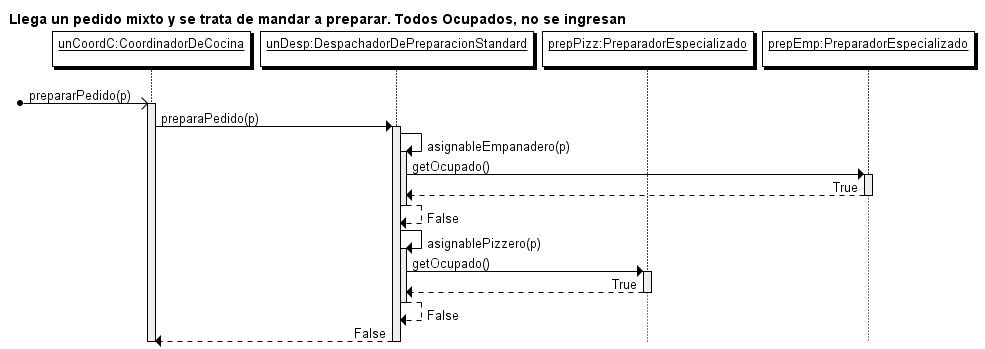
\includegraphics[height=6cm]{./figuras/mandanPrepararMixtoYEmpiezanNada.png}
\caption{Solicitud de preparacion de un pedido mixto cuando ambos maestros estan ocupados}
\end{figure}

Otro caso es aquel en el que uno de los maestros si esta dispuesto a comenzar la preparaci�n del pedido. En este caso, el pedido se encola para el empanadero (porque era mixto) pero comienza a preparse para el pizzero. Al hacerlo es necesario guardar alguna informaci�n sobre el pedido. Por ejemplo registrar que es mixto y que por lo tanto antes de estar listo se deben preparar los dos subpedidos (empanadas y pizzas). Y recordar que ese es el pedido que el pizzero esta preparando. Luego se entregan los subproductos a preparar al preparador y se notifica mediante el return que el pedido no debe quedar en la cola de ingreso, sino en preparaci�n.

\begin{figure}[H]
\centering
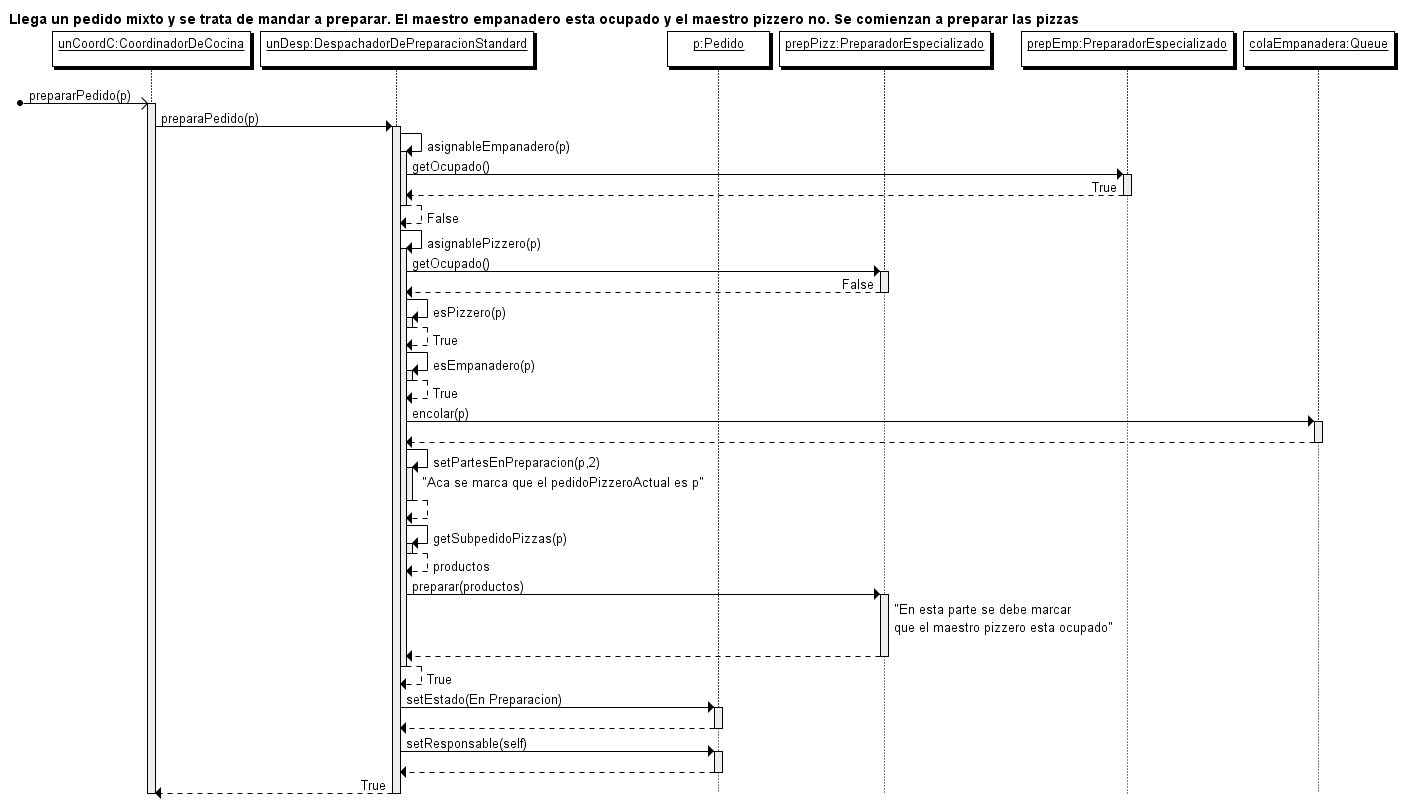
\includegraphics[height=10cm]{./figuras/mandanPrepararMixtoYEmpiezanPizzas.png}
\caption{Solicitud de preparacion de un pedido mixto cuando el maestro pizzero esta disponible}
\end{figure}

Finalmente podria ocurrir que ambos maestros esten ociosos, porque no habia ningun pedido en la pizzeria esperando por ser preparado. Y al llegar un nuevo pedido ambos comiencen a preparalo. La situaci�n es similar al caso anterior, pero en este caso no se encola el pedido, sino que se notifica a ambos preparadores para que estos luego realicen la notificaci�n.

\begin{figure}[H]
\centering
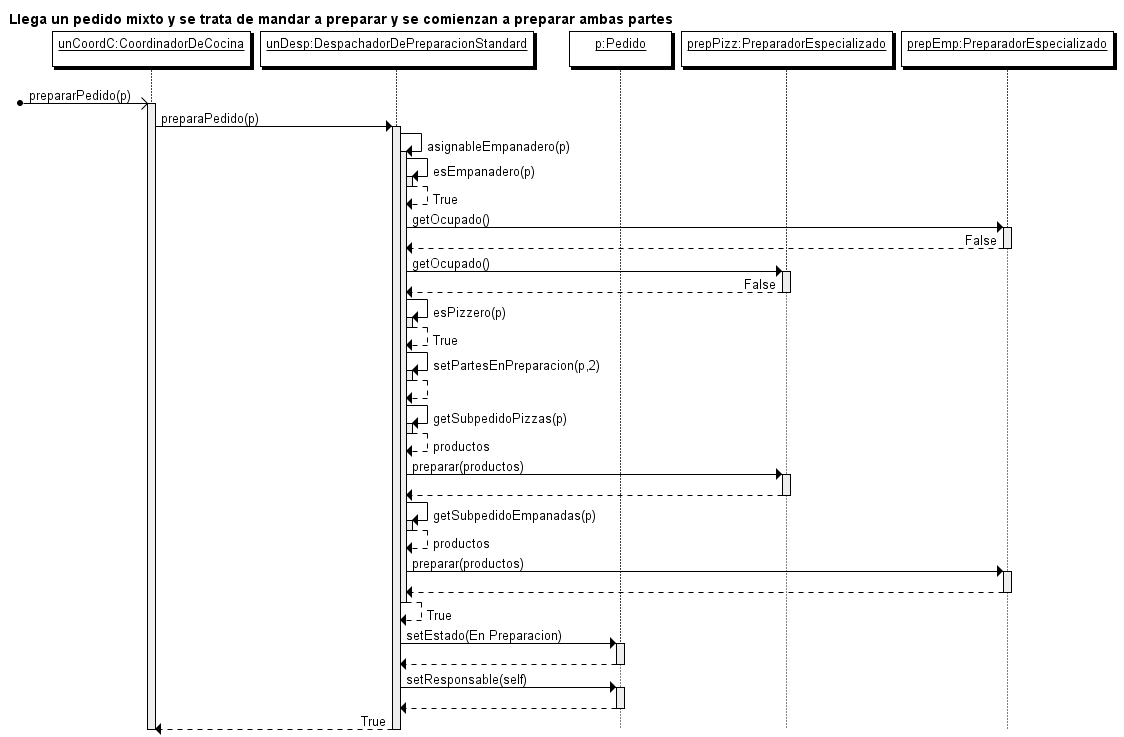
\includegraphics[height=11cm]{./figuras/mandanPrepararMixtoYEmpiezanAmbos.png}
\caption{Solicitud de preparacion de un pedido mixto cuando ambos maestros estan disponibles}
\end{figure}

\subsubsection{Terminancion de preparaci�n}
Cuando se indica que se termino de preparar una parte de un pedido, hay que seleccionar un nuevo pedido para poner a preparar. El despachador busca entonces en su cola interna y si esta esta vacia pide al coordinador de cocina que le consiga un pedido que contenga cierto tipo de producto. Este pasa la llamada al controlador de ingreso, que busca un pedido con el tipo pedido y en caso de encontrarlo lo devuelve. 

Ademas si el pedido entero termino de prepararse hay que enviarlo a cocinar, para ello se llama al corrdinador de cocina que deriva el pedido al despachador de coccion.

En el siguiente diagrama modelaremos el escenario en el que terminan de prepararse pizzas de un pedido, se consiguen mas pizzas en la cola interna y se pasan al preparador

\begin{figure}[H]
\centering
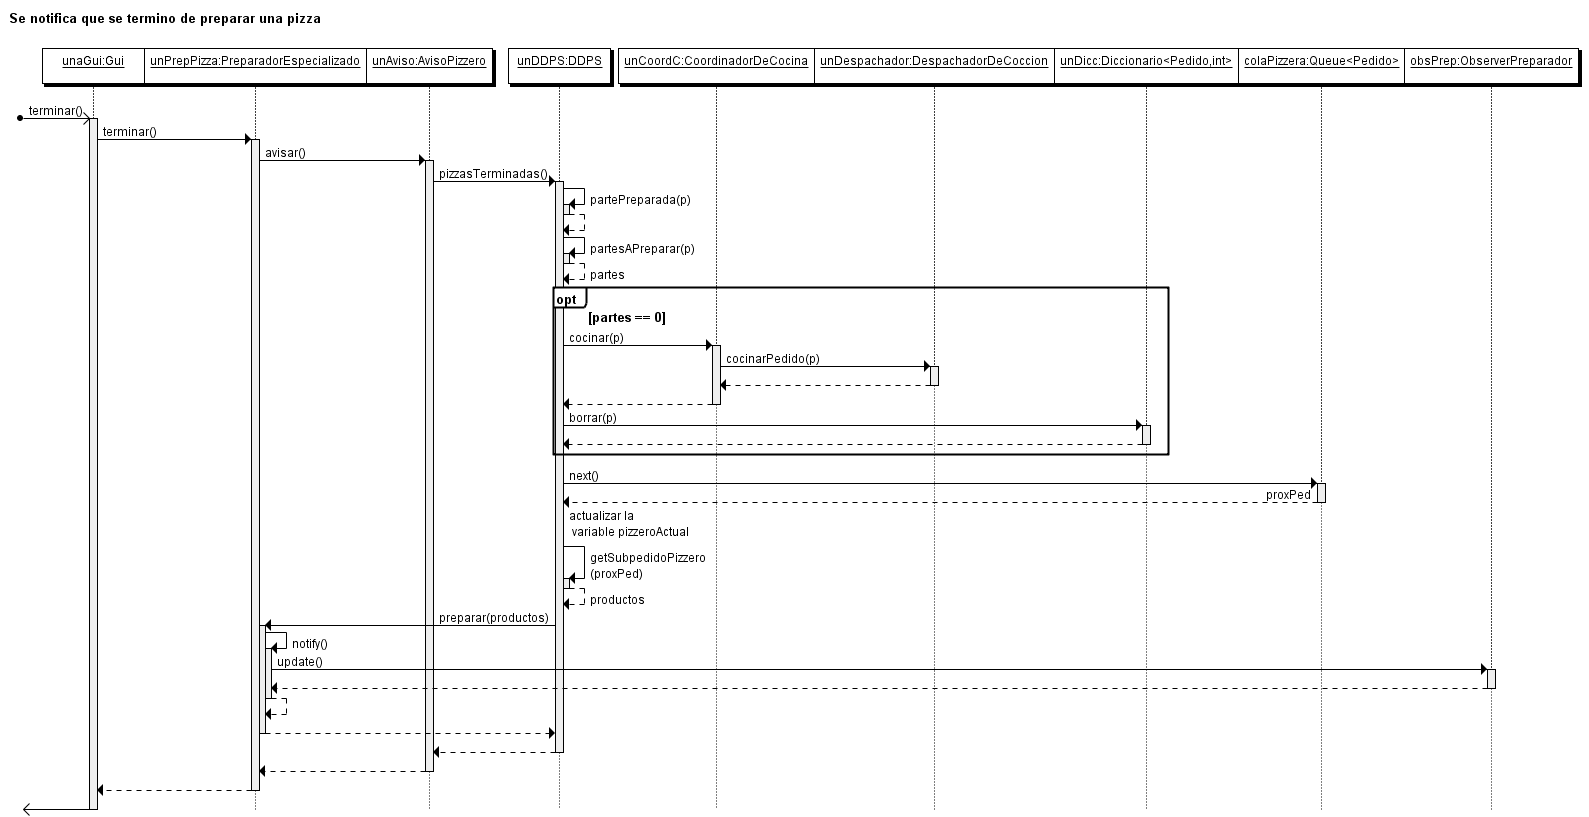
\includegraphics[height=8cm]{./figuras/terminarPreparacionPizza.png}
\caption{}
\end{figure}

Si la cola no estaba vacia, hay que buscar un pedido en la cola de ingreso. En este escenario modelamos esa alternativa.

\begin{figure}[H]
\centering
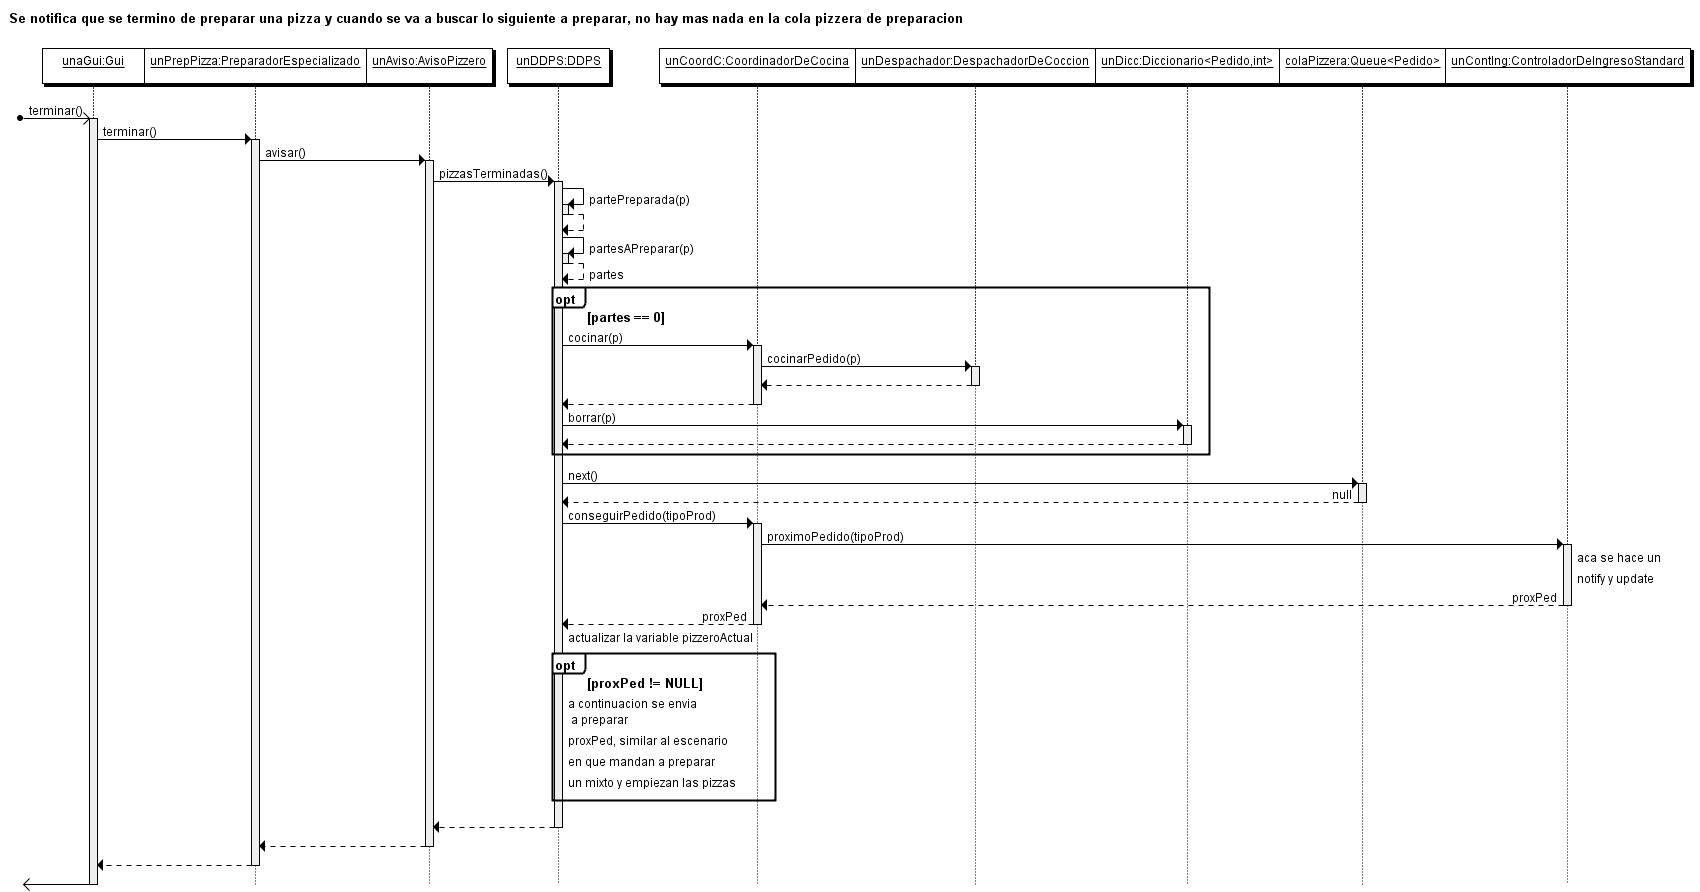
\includegraphics[height=8cm]{./figuras/terminarPreparacionPizzaYColaPizzeraVacia.png}
\caption{}
\end{figure}

\subsubsection{Ingreso de pedidos al horno}
Luego de ser preparados los pedidos pasan a traves del coordinador de cocina hacia el despachador de coccion. Este despachador es quien se encarga de manejar las colas de los hornos segun alguna politica. En particular en este trabajo consideraremos la politica normal y la politica agil, las cuales fueron debidamente especificadas en el trabajo anterior.

Basicamente ambas politicas, o despachadores tienen una estructura interna similar. Se utiliza un diccionario de numero de modulo a pedido que lo ocupa, para cada horno, hay dos colas de pedidos, pueden ser listas, ya que se por ejemplo se busca dentro de ellas, un diccionario que permite saber que partes faltan cocinar de un pedido y finalmente una variable de estado (2 en el caso de la politica agil) que permiten conocer que pedido esta a mitad de coccion, con elementos sin cocinar, y elementos cocinados o dentro del horno (la politica agil necesita 2 de estas variables ya que puede haber un pedido grande y un pedido chico en esta condicion).


%TODO: tal vez este no es el lugar para tantos detalles
Luego de terminar la preparacion de un pedido, el despachador invoca al coordinador, el cual a su vez llama al despachador de cocci�n. En un primer escenario a considerar, el pedido llega al despachador y como no hay lugar para entrar a su horno, se lo encola. Antes de encolarlo, se invoca al fraccionador, correspondiente al controlador del horno del pedido, para que separe al pedido en grupos de productos que se pueden colocar en un modulo. Es decir si el pedido es 3 pizzas y 3 empanadas y entran 2 empanadas por modulo y una pizza por modulo, una posible separacion de los productos del pedido es \{ 1 pizza, 1 pizza, 1 pizza, 2 empanadas, 1 empanada \}

En este escenario se asume que el horno 1 es el asignado al pedido.

%TODO: colocar el pseudocodigo del despachador

El diagrama de secuencia resultante es el siguiente:

\begin{figure}[H]
\centering
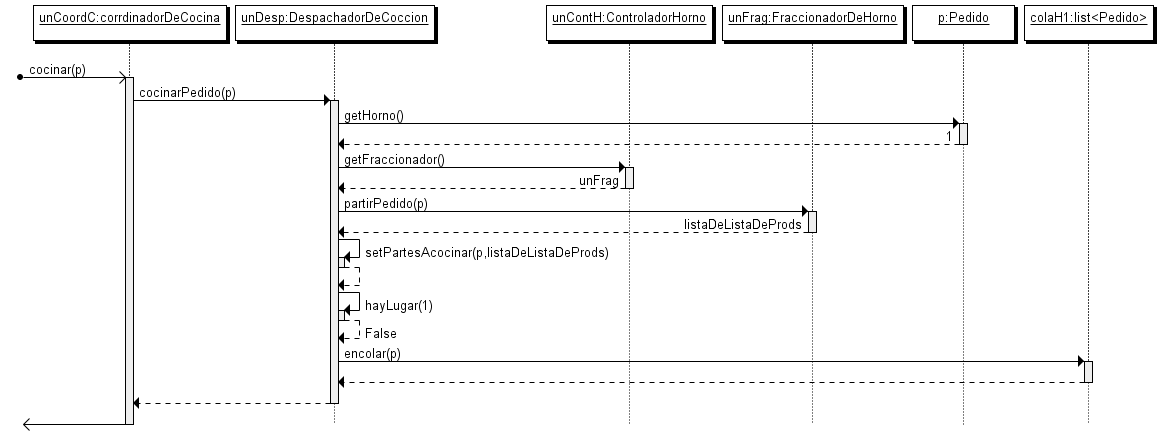
\includegraphics[height=8cm]{./figuras/llegaCocinarYseEncola.png}
\end{figure}

Otro escenario a considerar, comienza de igual manera que el anterior, pero esta vez si hay lugar en el horno para que el pedido entre. Lo que se hace es meter una parte del pedido en algun modulo libre, esto se repite mientras queden modulos libres o se termine el pedido. Por simplicidad en este escenario consideramos el caso donde solo habia un modulo libre. Una vez hecho eso, lo que ocurre es que se actualiza el estado interno. Por eso en este diagrama, al igual que en el anterior hay muchos automensajes, los cuales se deben a la gran cantidad de informaci�n interna que se necesita para mantener las politicas de acceso a los hornos.

\begin{figure}[H]
\centering
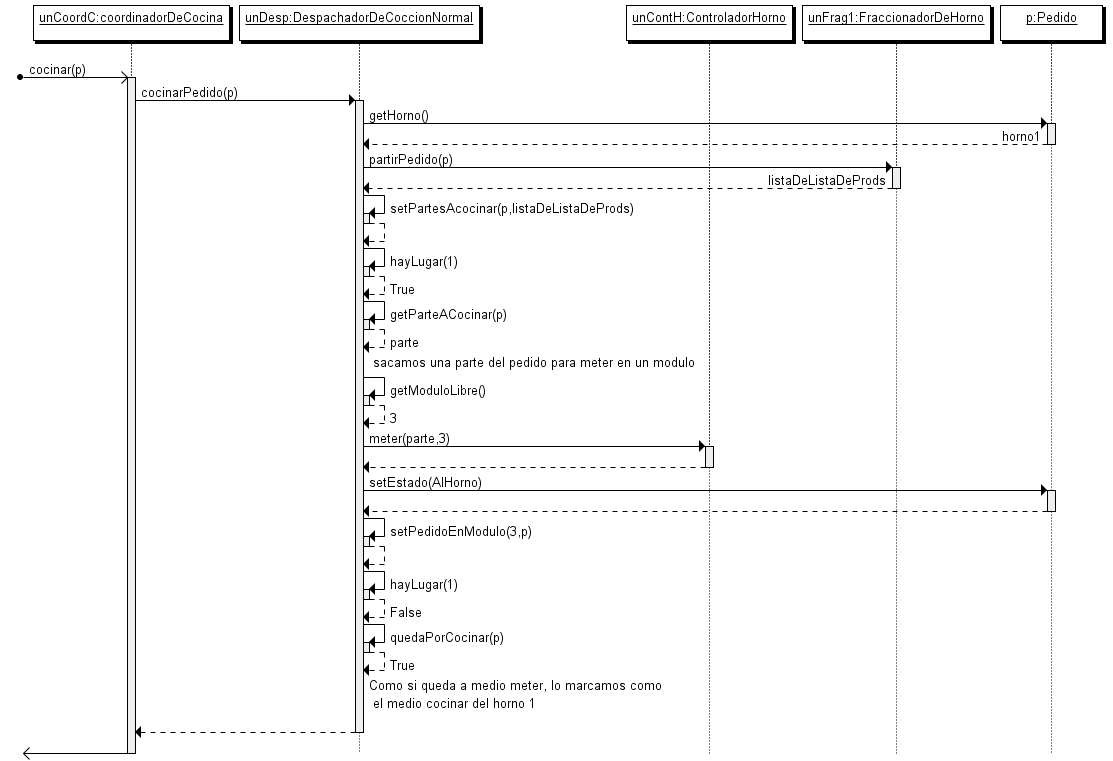
\includegraphics[height=8cm]{./figuras/llegaCocinarYNoseEncola.png}
\end{figure}

Queremos notar que estos escenarios aplican tambi�n para la politica agil, ya que los pedidos que llegan pueden quedarse encolados si no hay lugar (independientemente de si son agiles o no) y por otro lado pueden entrar si hay lugar libre, pero si hay lugar libre entran porque la cola es en esencia \textit{FIFO} en estas circunstancias, es decir si hay lugar vacio y solo hay un pedido, como se busca maximizar el uso del horno, se ingresa al mismo mas alla de su condicion de chico o grande. Nada impide que mas adelante se implemente una nueva politica que trate de hacer por ejemplo mas corto primero con conocimiento futuro, de modo que, por ejemplo use una cierta probabilidad $p$ para decidir si pone al pedido recien llegado al horno o no.

El fraccionado del pedido solo separa el pedido en bloques que entren en un modulo. El siguiente pseudocodigo permite ver como se hace.

\begin{algorithm}[H]
\caption{parte los productos de un pedido en grupos de productos que entran en un modulo}
\begin{algorithmic}[1]
\PARAMS{p:Pedido a partir}
\STATE res = $[]$
\STATE pizzas del pedido = [pr for p.productos if pr.tipoProd = Pizza]
\WHILE{ halla mas pizzas en pizzas del pedido que la cantidad de pizzas que entran en el modulo}
\STATE tomar A $\subset$ pizzas del pedido con $\sharp A ==$ pizzas que entran en el modulo
\STATE res += A
\STATE pizzas del pedido -= A
\ENDWHILE
\IF{ $\sharp$ pizzas del pedido $\neq$ 0}
\STATE res += pizzas del pedido
\ENDIF
\STATE empanadas del pedido = [pr for p.productos if pr.tipoProd = empanada]
\WHILE{ halla mas empanadas en empanadas del pedido que la cantidad de empanadas que entran en el modulo}
\STATE tomar A $\subset$ empanadas del pedido con $\sharp A ==$ empanadas que entran en el modulo
\STATE res += A
\STATE empanadas del pedido -= A
\ENDWHILE
\RETURN res
\end{algorithmic}
\end{algorithm}

\subsubsection{Fin de coccion de una parte}
%FIXME: diagramas obsoletos porq cambio el md
Hasta ahora solo consideramos cuando los pedidos entran al despachador provenientes de la etapa de prepraci�n. Consideremos entonces que ocurre cuando se notifica la terminaci�n de la cocci�n de una parte que estaba en el horno.

Supongamos una politica normal, y que la parte del pedido que sale no es lo ultimo que quedaba por cocinarse. Para determinar si un pedido se termino de cocinar, se pregunta si queda alguna parte por cocinar y si hay alguna en el horno, si ambas respuestas son negativas, se termino de cocinar. Notar que no se esta intentando saber que partes fueron cocinadas, sino cuantas faltan. Otra nueva politica podria interesarse en tener un control mas estricto, por ejemplo para informar de forma mas precisa el estado de un pedido que es al horno.

La notificaci�n de que una parte se termino de preparar la recibe el controlador de horno, el cual recibe que modulo se liber�. El controlador pasa el mensaje al despachador, el cual actualiza su estado en funci�n de este evento y busca si puede poner a cocinar algo.

Lo que hace el despachador normal es buscar si hay un pedido a medio cocinar, es decir con partes sin cocinar y fuera del horno. Si hay uno se toma una parte de ese. Podria ocurrir que al pedido a medio cocinar solo le quedaba esa parte por cocinar, en cuyo caso ahora no hay ningun pedido a medio cocinarse en ese horno.�

Si no habia ninguno a medio preparar toma el proximo pedido de la cola y busca alguna de sus partes para enviar al controlador de horno. Este nuevo pedido podr�a pasar a ser el nuevo pedido a medio cocinar.

Si no habia ningun pedido en la cola tampoco, no tiene nada que hacer luego de actualizar su estado.

\begin{figure}[H]
\centering
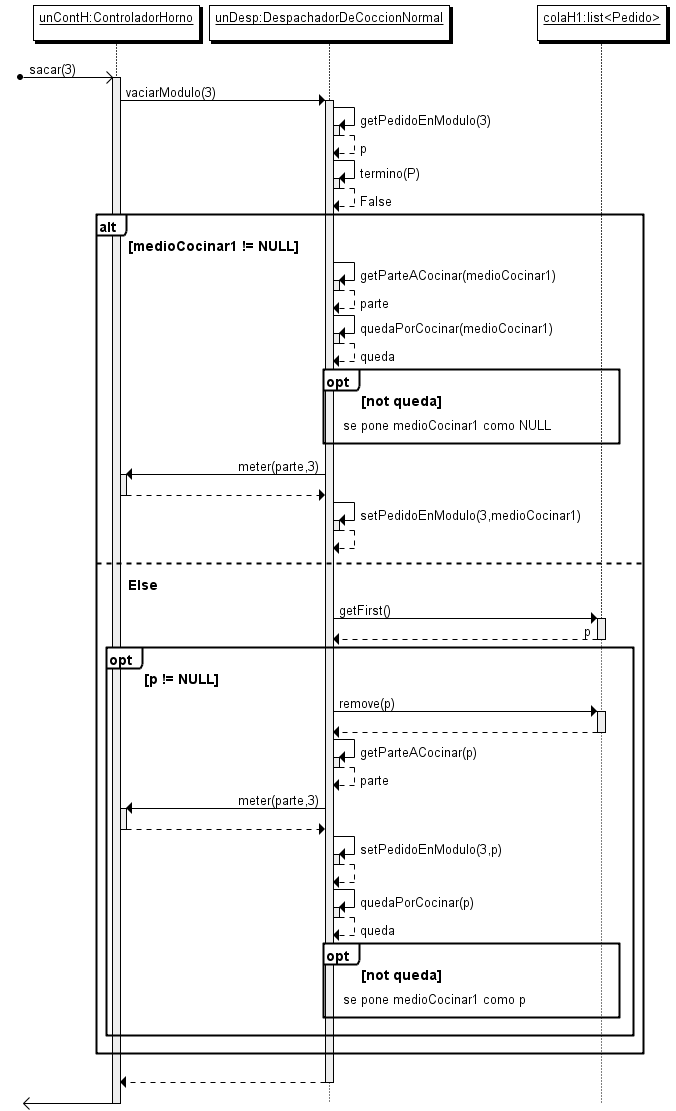
\includegraphics[height=18cm]{./figuras/saleUnPedidoNormalNoTermina.png}
\end{figure}

Notar que si medioCocinar es distinto de NULL tiene al menos una parte que se puede cocinar, por ende es valida la llamada al metodo $getParteACocinar$.

\begin{algorithm}[H]
\caption{Determina que meter en el horno segun politica normal}
\begin{algorithmic}[1]
\REQUIRE{hay a lo sumo un unico pedido a medio cocinar}
\ENSURE{se decide el proximo pedido a preparar segun lo especificado en el tp1 (salvando el hecho de que se vacia de a un modulo por vez)}
\IF{hay un pedido a medio cocinar}
\STATE productos a meter = tomar un grupo de productos del pedido para llenar un modulo (o lo mas que se pueda si no alcanza) \COMMENT{ver algoritmo de division del pedido}
\IF{eso era lo ultimo que quedaba por poner del pedido a medio cocinar}
\STATE poner pedido a medio cocinar = $\textcolor{ForestGreen}{\bot}$
\ENDIF
\RETURN productos a meter 
\ELSE
\STATE buscar en la cola el primer pedido
\IF{hay alguno}
\STATE productos a meter= tomar un grupo de productos del pedido sacado de la cola
\IF{queda algo de ese pedido por meter}
\STATE poner al pedido como pedido a medio cocinar
\ENDIF
\RETURN productos a meter
\ELSE
\RETURN $\textcolor{ForestGreen}{\bot}$
\ENDIF
\ENDIF
\end{algorithmic}
\end{algorithm}


En el escenario donde la politica es agil, la situaci�n es similar, en particular en el caso de que el modulo que se vacia no es agil, es el mismo procedimiento. Si el modulo que se vacia si es agil, el funcionamiento se modifica. En vez de intentar meter el pedido a medio cocinar se busca el pedido chico a medio cocinar. Si no hay, lo que se hace es buscar si hay algun chico en la cola, cuando lo encuentra el proceso es similar al escenario anterior, solo que este pedido puede llegar a ser el chico a medio cocinar. Si tampoco lo encuentra, busca como si fuera una politica normal. Esto nos permite ver como la politica agil, frente a la ausencia de pedidos chicos, es exactamente igual a la politica normal.

\begin{figure}[H]
\centering
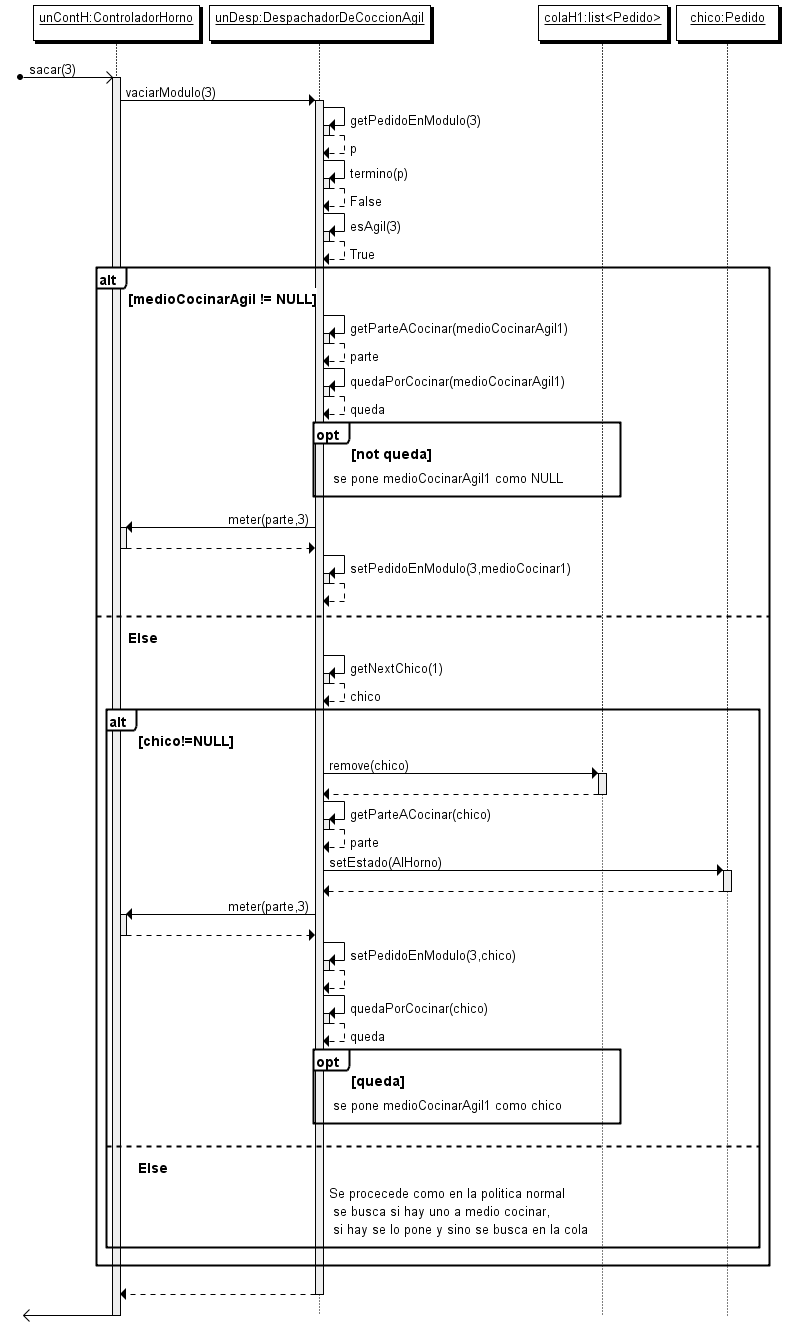
\includegraphics[height=21cm]{./figuras/saleUnPedidoAgilNoTermina.png}
\end{figure}

\begin{algorithm}[H]
\caption{determina como llenar un modulo agil que se vacia}
\begin{algorithmic}[1]
\REQUIRE{hay a lo sumo un unico pedido a medio cocinar normal y uno chico a medio cocinar}
\ENSURE{se decide el proximo pedido a preparar segun lo especificado en el tp1 (salvando el hecho de que se vacia de a un modulo por vez)}
\IF{hay un pedido chico a medio cocinar}
\STATE productos a meter = tomar un grupo de productos del pedido chico para llenar un modulo (o lo mas que se pueda si no alcanza) \COMMENT{ver algoritmo de division del pedido}
\IF{eso era lo ultimo que quedaba por poner del pedido chico a medio cocinar}
\STATE poner pedido a chico a medio cocinar = $\textcolor{ForestGreen}{\bot}$
\ENDIF
\RETURN productos a meter
\ELSE
\STATE buscar en la cola el primer pedido chico
\IF{hay alguno}
\STATE productos a meter = tomar un grupo de productos que llenen un modulo
\IF{queda algo del pedido fuera del horno}
\STATE poner chico a medio cocinar = pedido
\ENDIF
\RETURN productos a meter
\ENDIF
\IF{hay algun producto en la cola}
\STATE tomar el primer pedido
\STATE productos a meter= tomar un grupo de productos del pedido sacado de la cola
\IF{queda algo de ese pedido por meter}
\STATE poner al pedido como pedido a medio cocinar
\ENDIF
\RETURN productos a meter
\ENDIF
\RETURN $\textcolor{ForestGreen}{\bot}$
\ENDIF
\end{algorithmic}
\end{algorithm}

\subsubsection{Fin de cocci�n de un pedido}
Cuando una parte termina de cocinarse, el despachador se pregunta si el pedido finaliz� de cocinarse. En el caso en el que afirmativamente terminara de cocinarse, se debe pasar el pedido a la cola de listos. El diagrama de secuencias presente a continuaci�n permite modelar este escenario, donde un pedido termina de cocinarse.

Al terminar de cocinar un pedido debe borrarse el pedido del diccionario de pedidos y pasarlo a la cola de listos (pasando por los coordinadores). No modelaremos de nuevo como elegir el proximo pedido, sino que modelaremos hasta que el pedido llega a la cola de listos.

\begin{figure}[H]
\centering
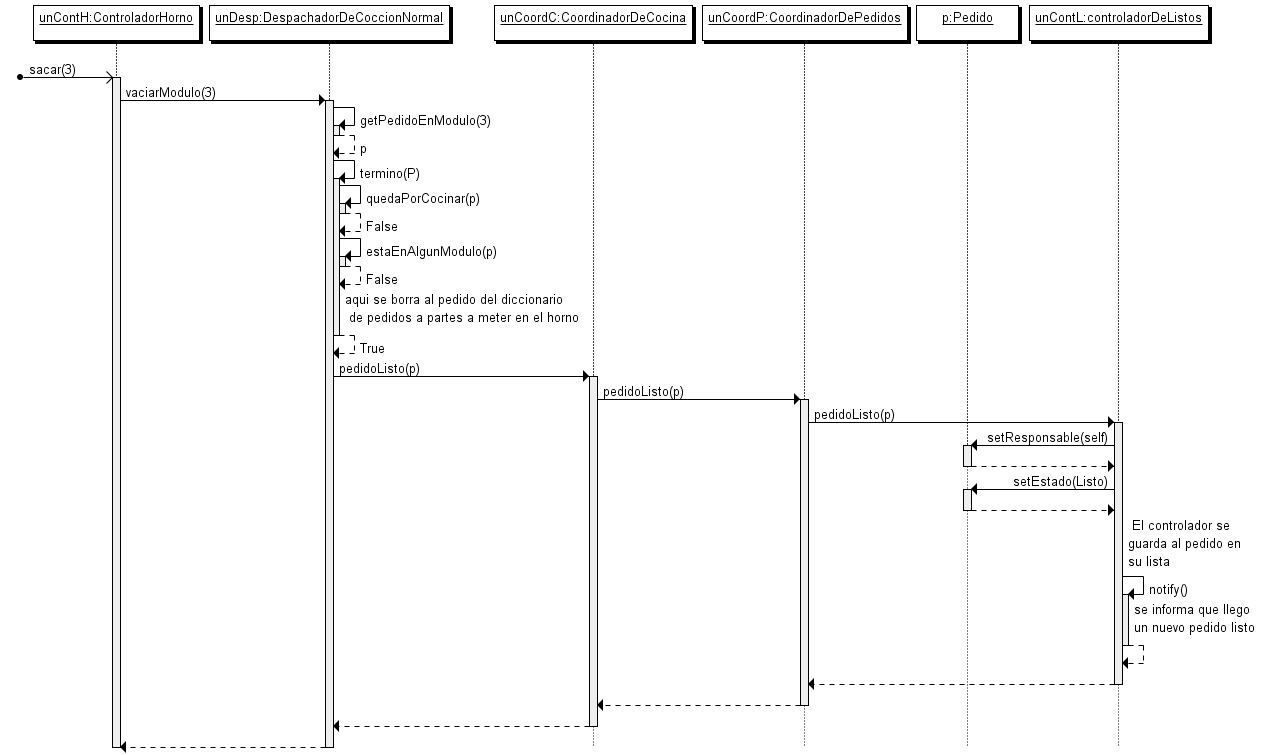
\includegraphics[height=10cm]{./figuras/finDeCoccion.png}
\end{figure}